\section{Numerical validation and claim boundaries}
\label{sec:numerical-validation}

We validate the deterministic identities before testing any scaling or timing
claim.  All nonlinear-kernel experiments use the prescribed RBF score and
quadrature weights; its length scale is fixed by the covariance model and is
never optimized from the reported test data.  Raw samples, configuration, and
failure-preserving summaries accompany this manuscript.

\paragraph{Algebra, RMT, and reduced DMFT.}
The weighted softmax/kernel identity has maximum relative residual
$7.859\times 10^{-16}$,
and no nonvacuous Ritz spectral certificate is violated.  Monte Carlo fixed
polynomial risk agrees with the exact trace formula to relative error
$0.007222$.  The
Marchenko--Pastur comparison is used only as a linear-Wishart control.  For the
normalized RBF operator we instead measure its own one- and two-resolvent
statistics; their penultimate/coarsest finite-size discrepancy ratio is
$0.1494$.
Thus these experiments support convergence of the probed kernel statistics,
not an unproved closed-form nonlinear deterministic equivalent.  The FS/RRS
time, depth, width/context, balanced-parameterization, and finite-task
isotropy slopes pass their prespecified finite-window tolerance and $R^2$
criteria.  Regression standard errors are reported diagnostically; deterministic
modal-truncation bias is not treated as sampling noise.

\begin{table}[H]
\centering
\caption{Measured log--log exponents against the reduced-theory values.}
\label{tab:scaling-exponents}
\begin{tabular}{lrrr}
\toprule
Law & measured & theory & $R^2$\\
\midrule
FS time & -0.3158
 & -0.3158
 & 1\\
RRS loss versus scale & -1.506
 & -1.5
 & 1\\
RRS time, $r=1$ & -0.4302
 & -0.4286
 & 1\\
RRS time, $r=5$ & -0.7928
 & -0.7895
 & 1\\
RRS width/context & -1.198
 & -1.2
 & 1\\
RRS depth & -1.558
 & -1.5
 & 1\\
Finite-task isotropy & -0.4967
 & -0.5
 & 0.9999\\
\bottomrule
\end{tabular}
\end{table}

\begin{figure}[H]
\centering
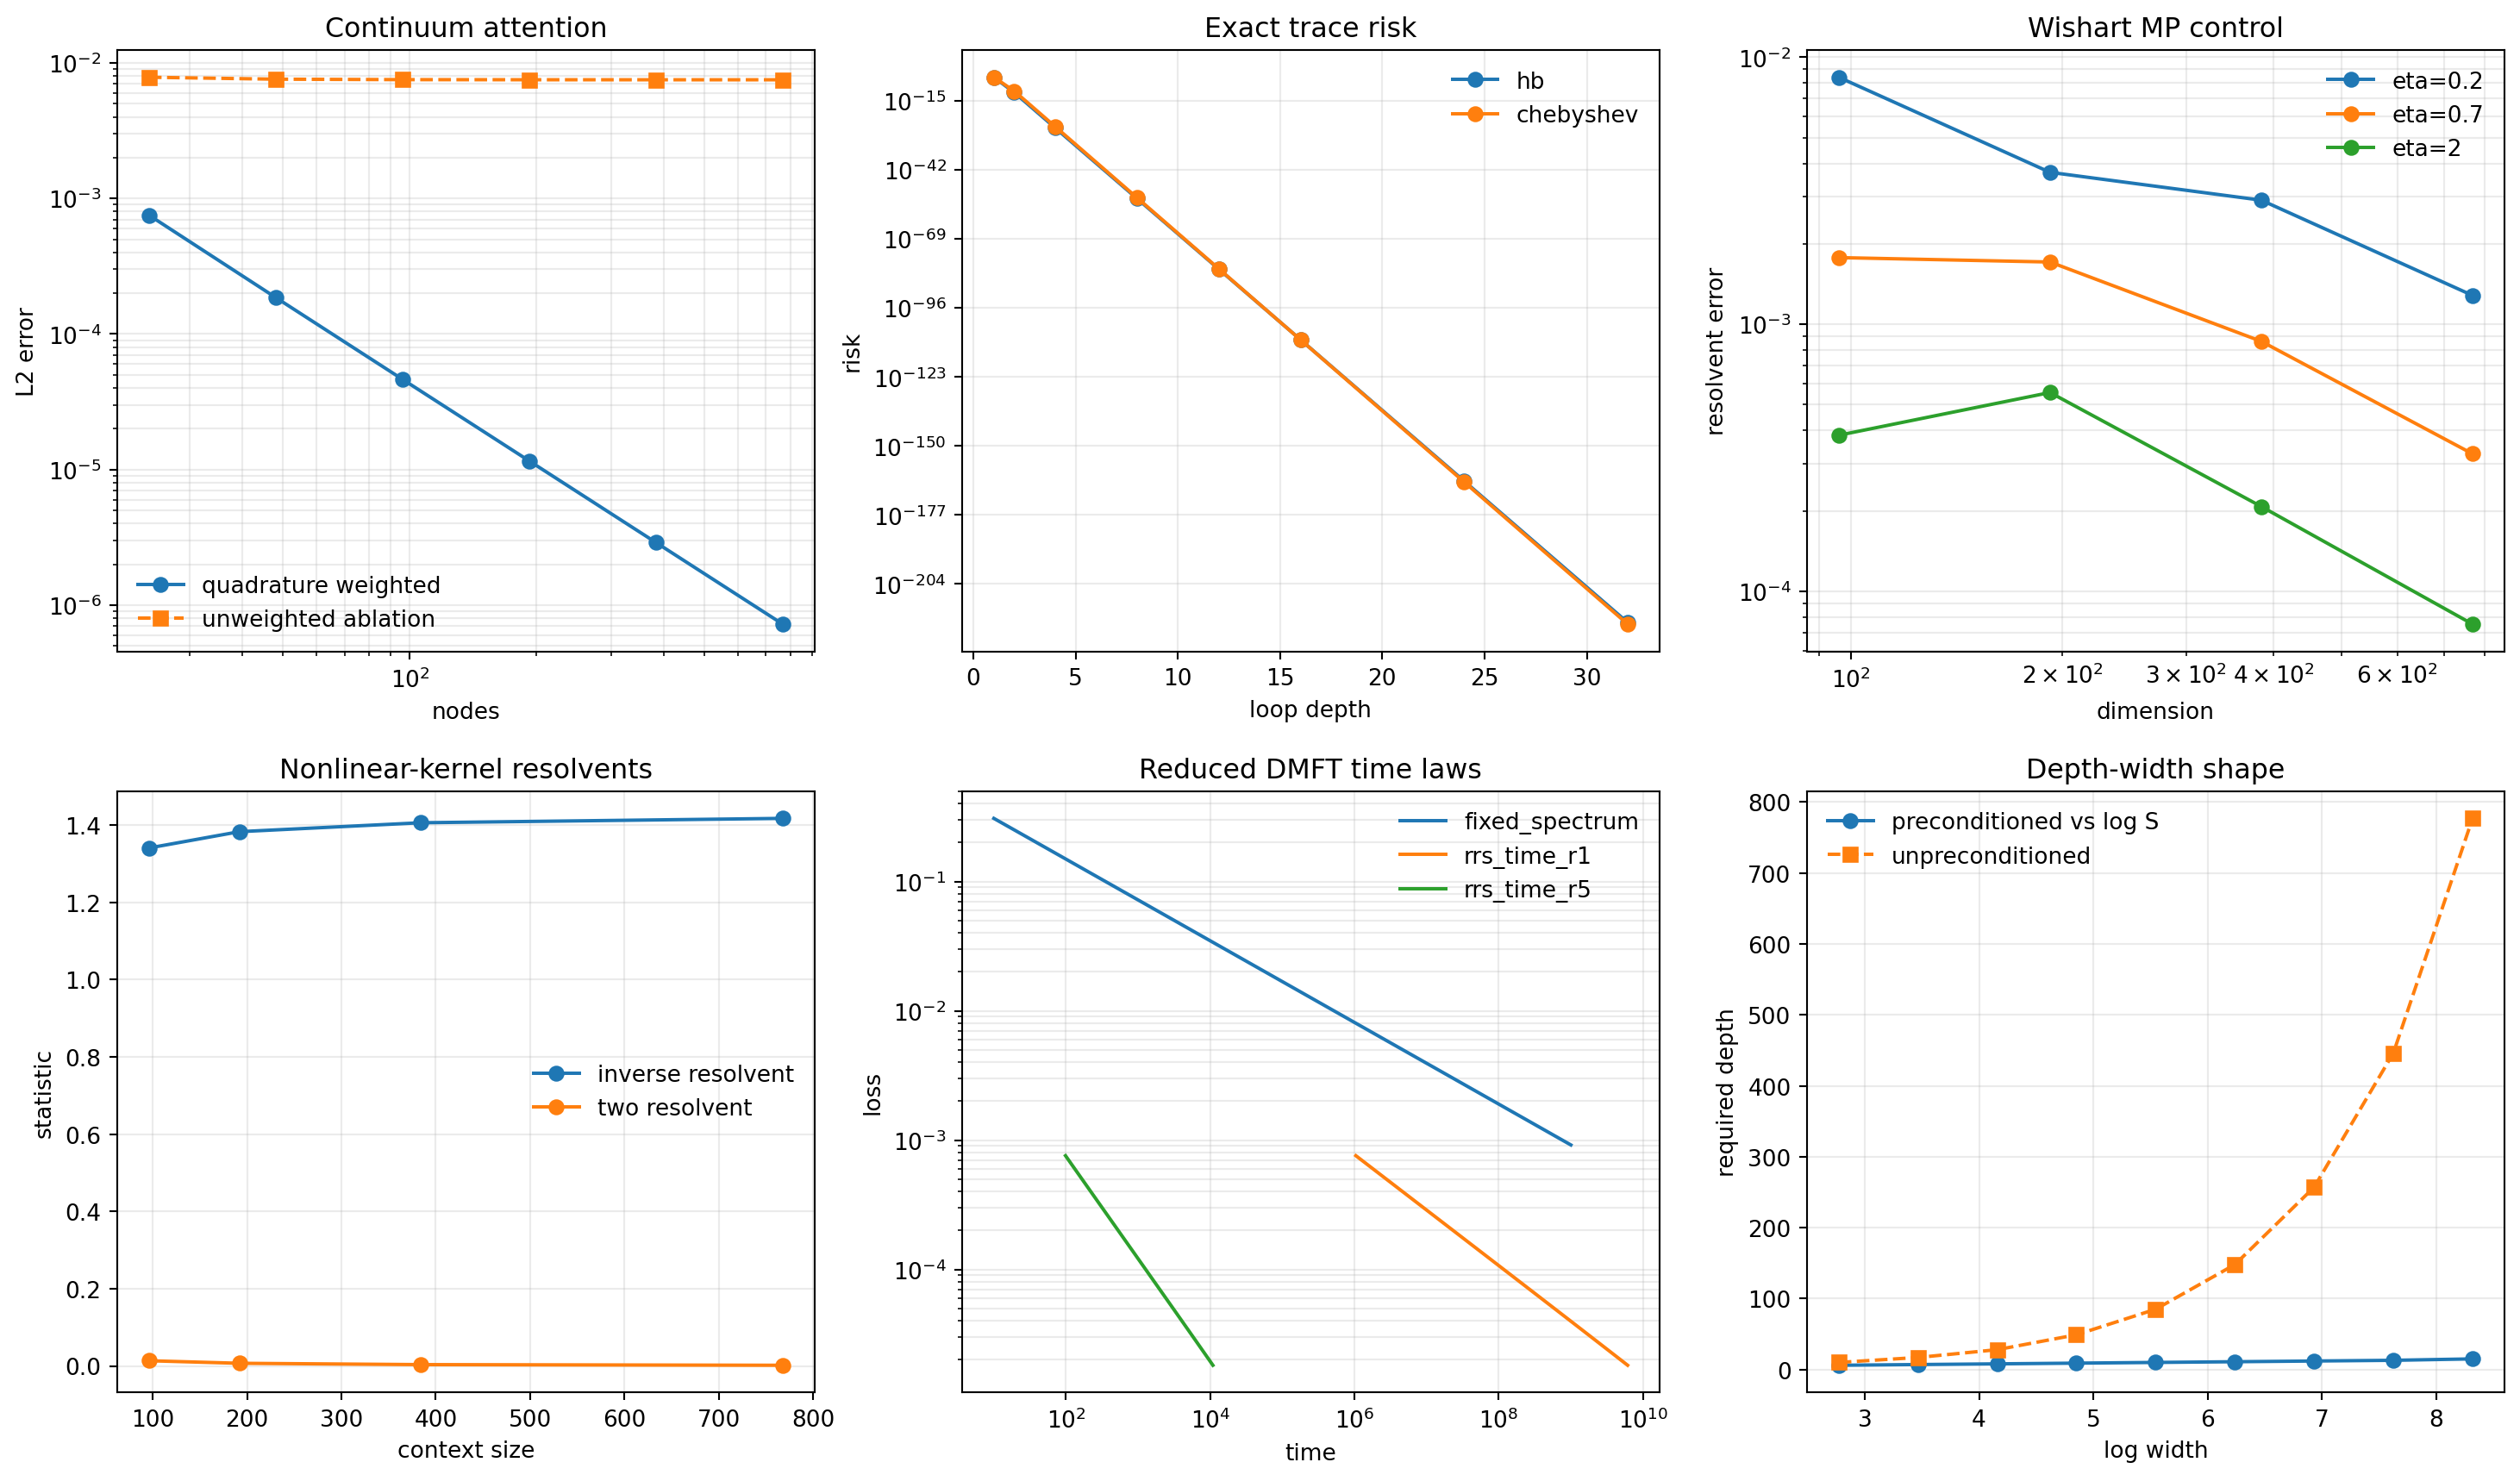
\includegraphics[width=0.98\linewidth]{experiments/transformers/kernel_matched_continuum_validation/results/theory/theory_validation_overview.png}
\caption{Algebraic, RMT, nonlinear-resolvent, reduced-DMFT, and
depth--width validations.  Marchenko--Pastur is shown only for the linear
control.}
\label{fig:theory-validation}
\end{figure}

\paragraph{Discretization covariance.}
On nonuniform meshes the lifted Ritz metric converges with fitted order
$2$ and
the transfer commutator with order
$2.437$.
Removing quadrature weights increases the finest-grid metric error by a factor
$4.037\times 10^{4}$.  This
directly separates continuum covariance from mere variable-length execution.

\begin{figure}[H]
\centering
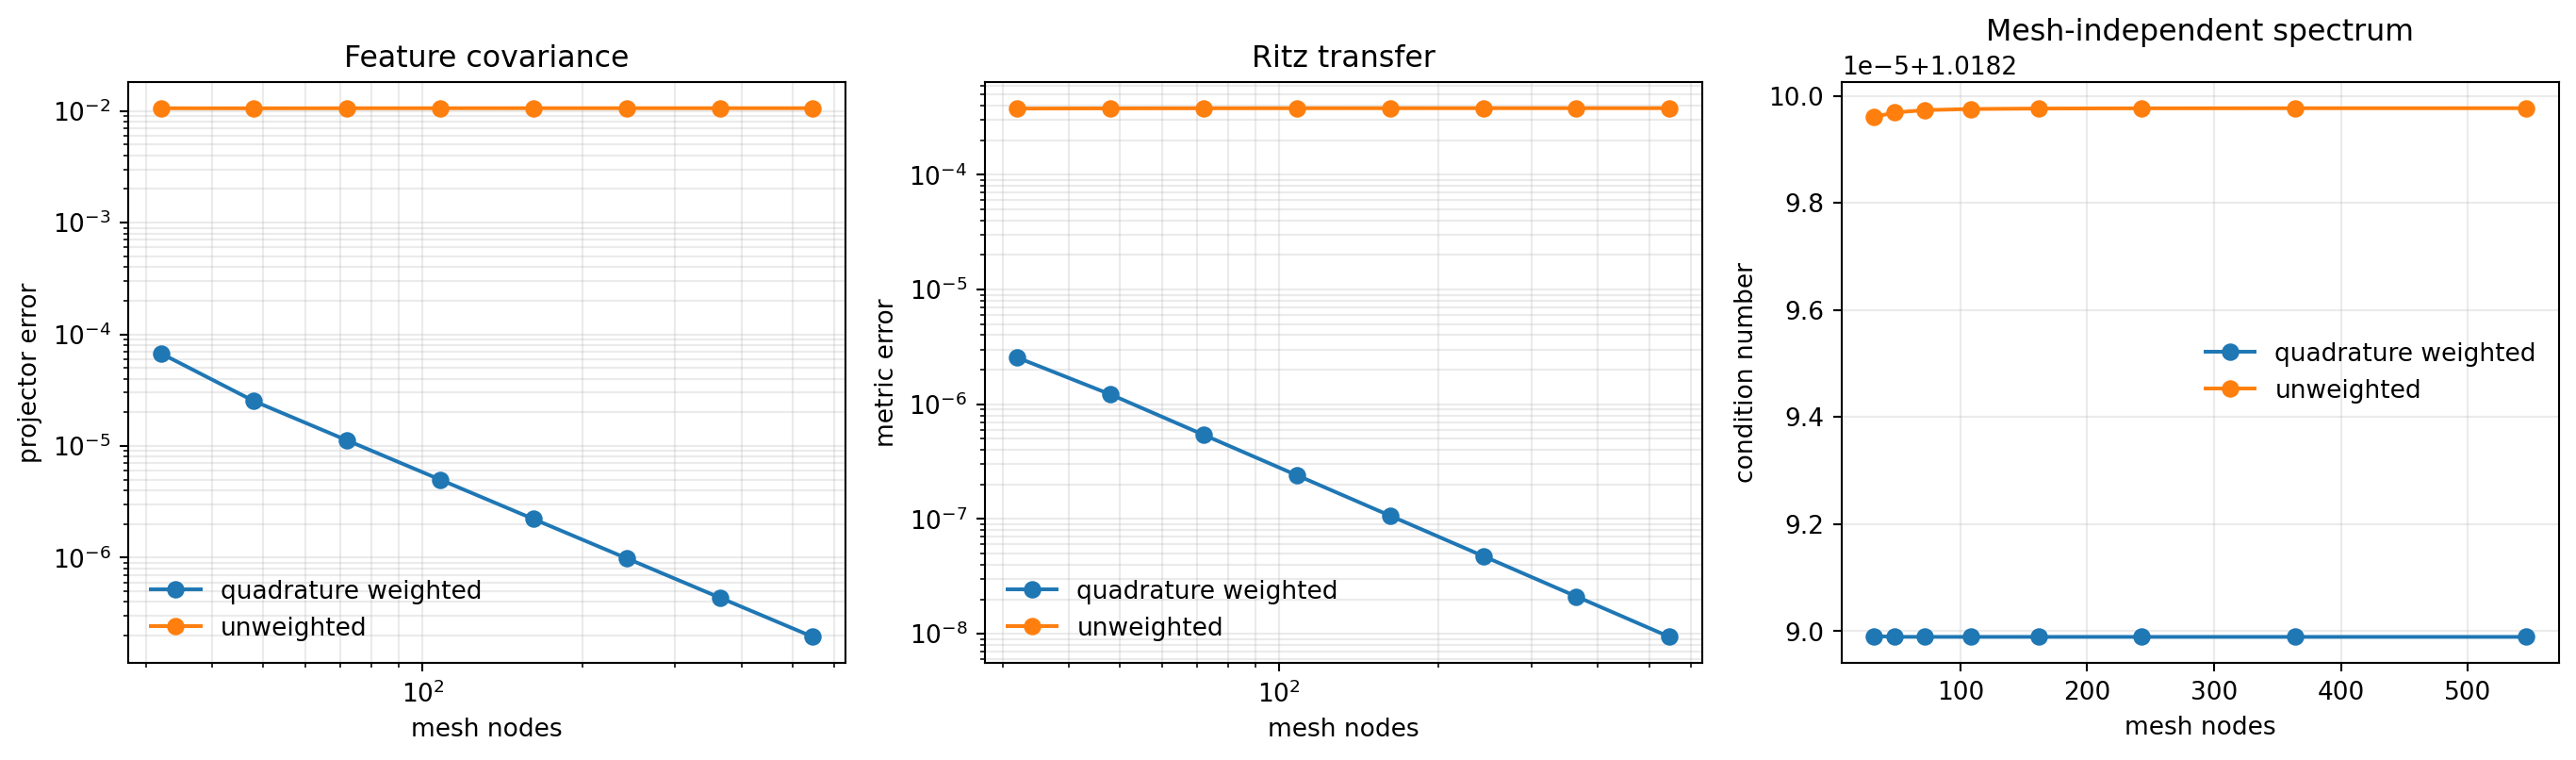
\includegraphics[width=0.82\linewidth]{experiments/transformers/kernel_matched_continuum_validation/results/discretization/discretization_validation.png}
\caption{Nonuniform-mesh transfer.  Quadrature weighting converges to one
lifted projector and Ritz metric, while the unweighted head retains a
sampling-measure bias.}
\label{fig:discretization-validation}
\end{figure}

\paragraph{Elliptic Bayesian inverse problem.}
We solve
$-\nabla\!\cdot(a_z\nabla u)+0.2u=m$ on the unit square with homogeneous
Dirichlet data.  The log-diffusion is a bounded random Fourier field and the
source covariance square root is
$W_z=\sigma_fI+\Phi_z\operatorname{diag}(d_z)\Phi_z^\top$, with a
task-dependent localized rank-24 component and a
nonzero floor.  Point observations and sparse elliptic solves produce the
prior-whitened posterior $H_z=I+U_zU_z^\top$.  The model-chosen RBF length
scale is compared with short- and long-scale ablations before one exact
block-power refinement and the Ritz construction.  The largest
standard sweep has $16384$ state unknowns and
$512$ observation tokens.  The contextual
kernel--Ritz metric reduces the effective condition number by a factor
$885.7$ and the
fixed four-HVP loops meet the common residual tolerance.  At this moderate
context, exact Woodbury is faster; its one-query total divided by kernel--HB is
$0.2137$.
Accordingly we make no universal speed claim against a structure-exploiting
Woodbury solve.

\begin{figure}[H]
\centering
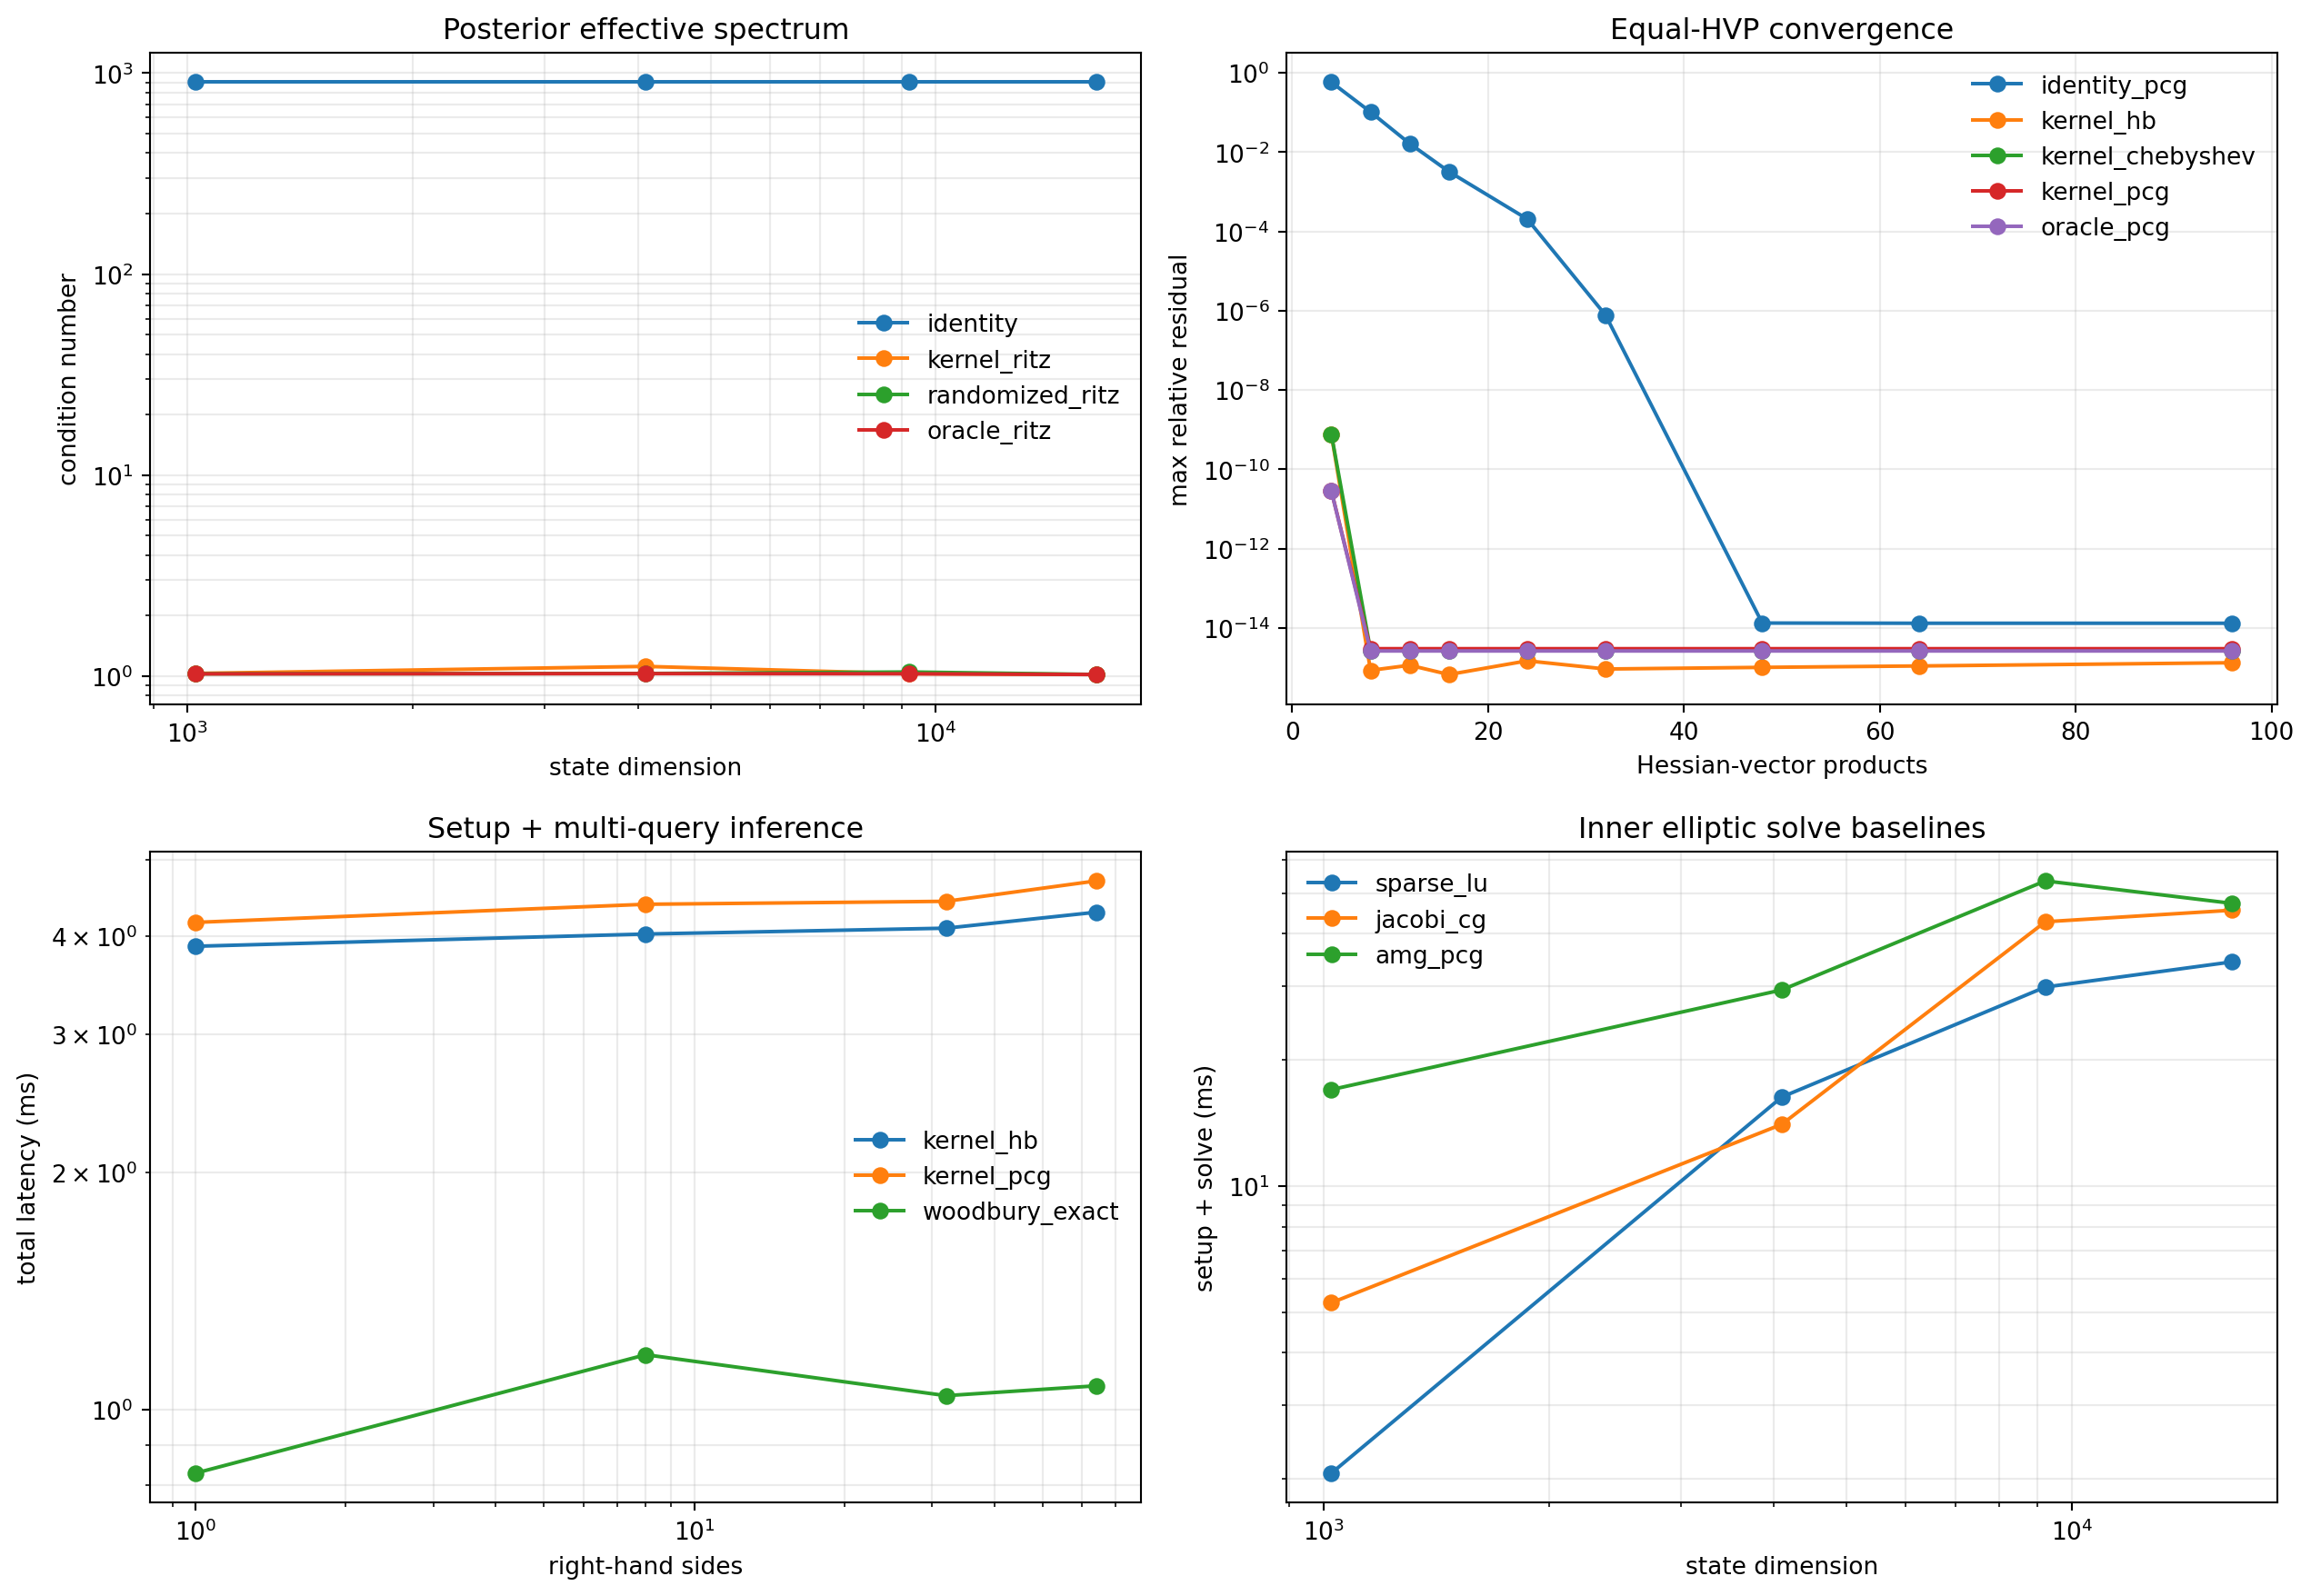
\includegraphics[width=0.90\linewidth]{experiments/transformers/kernel_matched_continuum_validation/results/pde/pde_validation_overview.png}
\caption{Variable-coefficient elliptic posterior validation: effective
spectra, equal-HVP convergence, multi-query timing, and sparse LU/Jacobi/AMG
inner PDE baselines.}
\label{fig:pde-validation}
\end{figure}

\begin{table}[H]
\centering
\caption{Long-context setup-plus-one-query latency on the same posterior
system on an NVIDIA H100 PCIe.  Parentheses give bootstrap 95\%
intervals from 11 repetitions.}
\label{tab:long-context-crossover}
\begin{tabular}{lrrr}
\toprule
Method & depth & latency (ms) & maximum relative residual\\
\midrule
Kernel--Ritz HB & 10 & 10.9
 [10.87,11.27]
 & $2.268\times 10^{-8}$\\
Exact Woodbury & --- & 24.03
 [23.38,24.26]
 & $1.541\times 10^{-15}$\\
Dense Cholesky & --- & 139.8
 [135.5,141.3]
 & $1.849\times 10^{-14}$\\
\bottomrule
\end{tabular}
\end{table}

At state dimension $N=16384$ and context length
$m=4096$, the measured dense/kernel median ratio is
$12.82$.
A nonoverlapping Woodbury crossover is also observed.
The admissible inference-speed statement is therefore restricted to the
measured context/query region and always includes feature construction.  PDE
assembly is a common context cost and is reported separately; AMG-PCG and
sparse LU are included as inner elliptic baselines.

\begin{figure}[H]
\centering
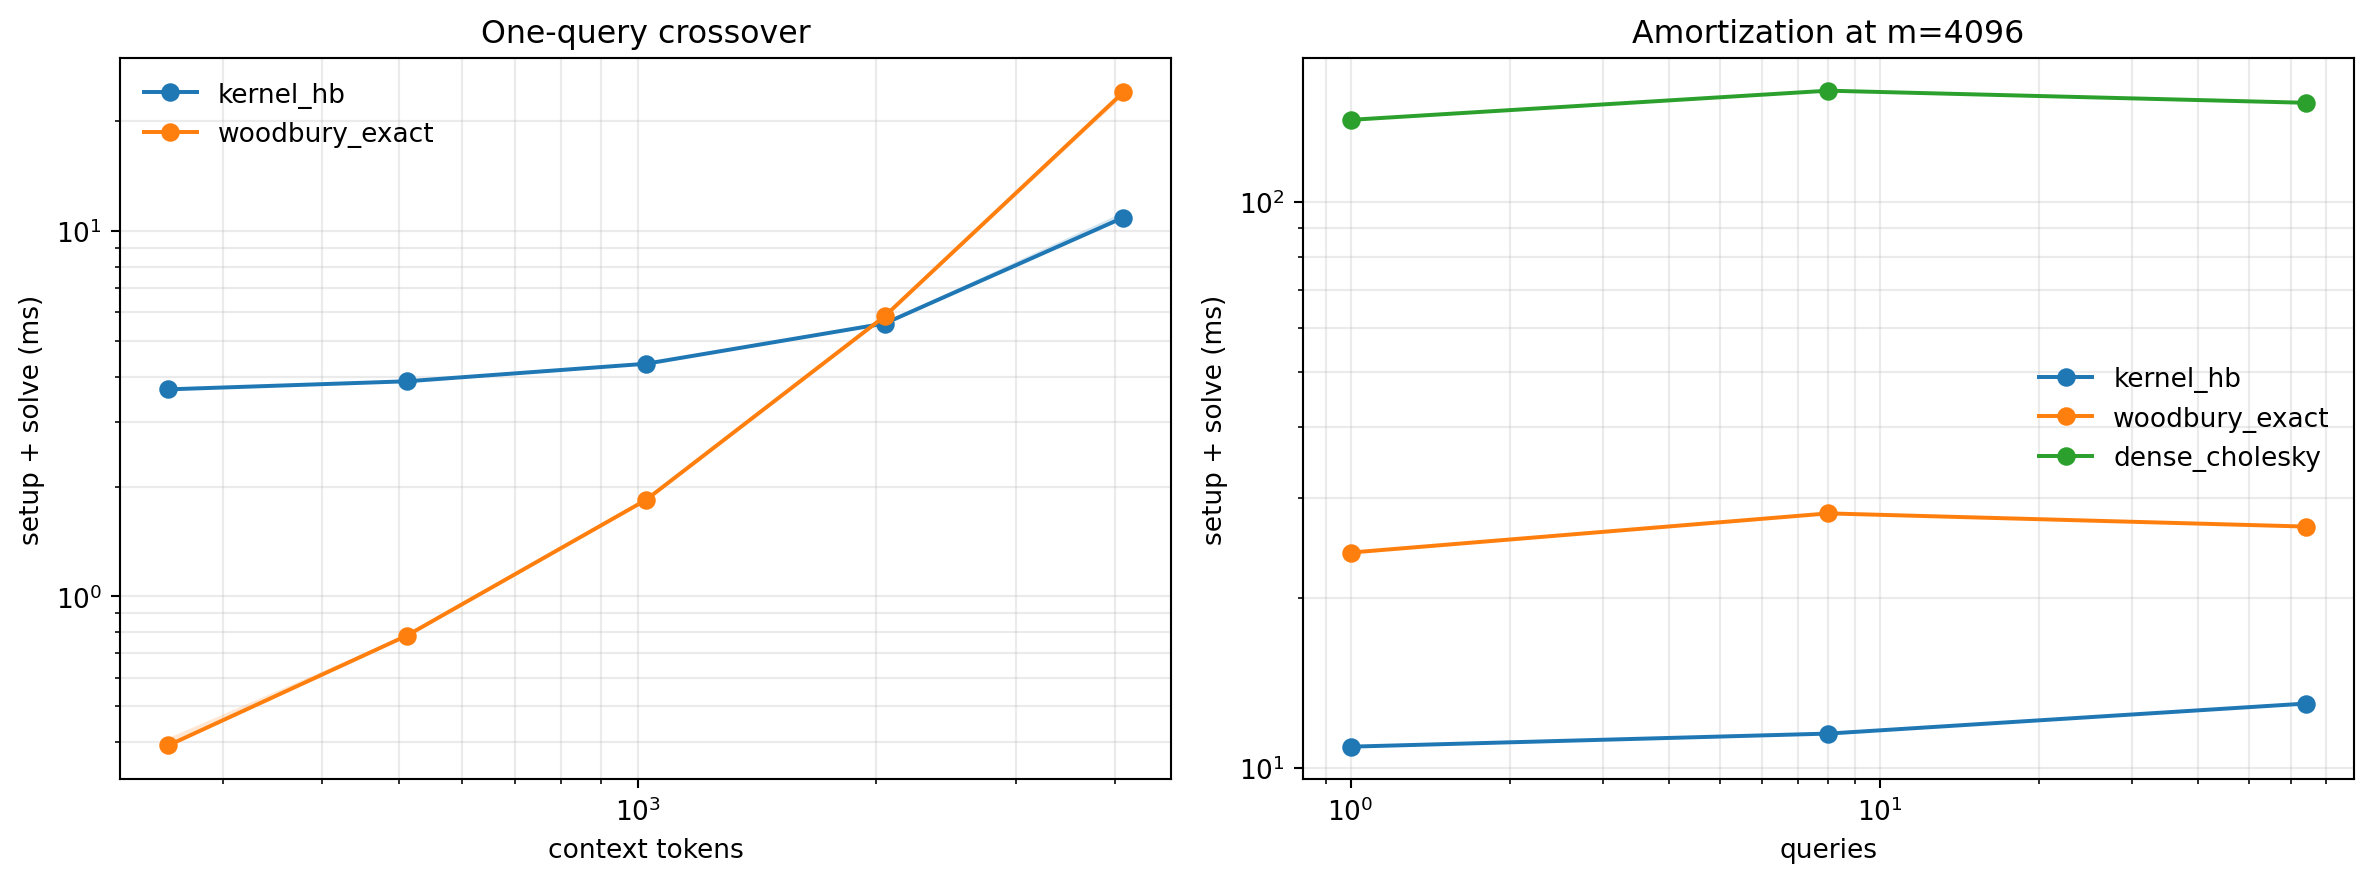
\includegraphics[width=0.82\linewidth]{experiments/transformers/kernel_matched_continuum_validation/results/crossover/long_context_crossover.png}
\caption{Setup-inclusive long-context crossover and multi-query
amortization.  Exact Woodbury is faster at short context; the compressed
kernel--Ritz loop crosses it only once the context is sufficiently long.}
\label{fig:long-context-crossover}
\end{figure}
\FloatBarrier
